% !TEX root =../prj4projektrapport.tex

\section{Trinskifter}
\label{sec:relae}
Ved projektets start fik gruppen udleveret en trintransformer\footnote{Projektdokumentation, 6.1, Valg af transformer}. Denne transformer har på primærside 24V og trin af 1V fra 0-8V på sekundærside. Disse forhold afgjorde skaleringen af systemet, se bilag C3 og C4 for billeder af transformer og tilhørende mærkeplade. 

De forskellige trin og dermed spændingsniveauer på sekundærside af transformeren er bestemt af antallet af tilkoblede viklinger. Det ønskede spændingsniveau hos forbrugeren er valgt til 4V, og det er i systemet muligt at skifte mellem trin 4V, 5V og 6V på trintransformeren. Disse tre trin gør det muligt at holde spændingen hos forbrugeren på $\pm$10$\%$ af 4V, når belastningen varierer.

\subsection{Design og implementering af relækredsløb}
Til at styre tilkoblingen af trin på transformeren er der designet et relækredsløb. Relæerne er sat til Normally Open og virker som kontakter, der slutter, når relæerne trækker, se bilag B-5. Kontaktrelæerne skal styres af en PLC, og skal derfor kunne holde til et 24VDC styresignal \footnote{Projektdokumentation, 8.4, Trinskifter}. Det færdige print med relæerne ses på figur \ref{fig:Relae}. De sorte bananstik kobles til henholdsvis trin 4V, 5V og 6V på transformeren. Øverst til ses pin, der kobles til Distributionslinjen. De tre pins nederst til venstre er til styresignal fra PLC og den fjerde er stelforbindelse for PLC. 

\begin{figure}[H]
	\centering
	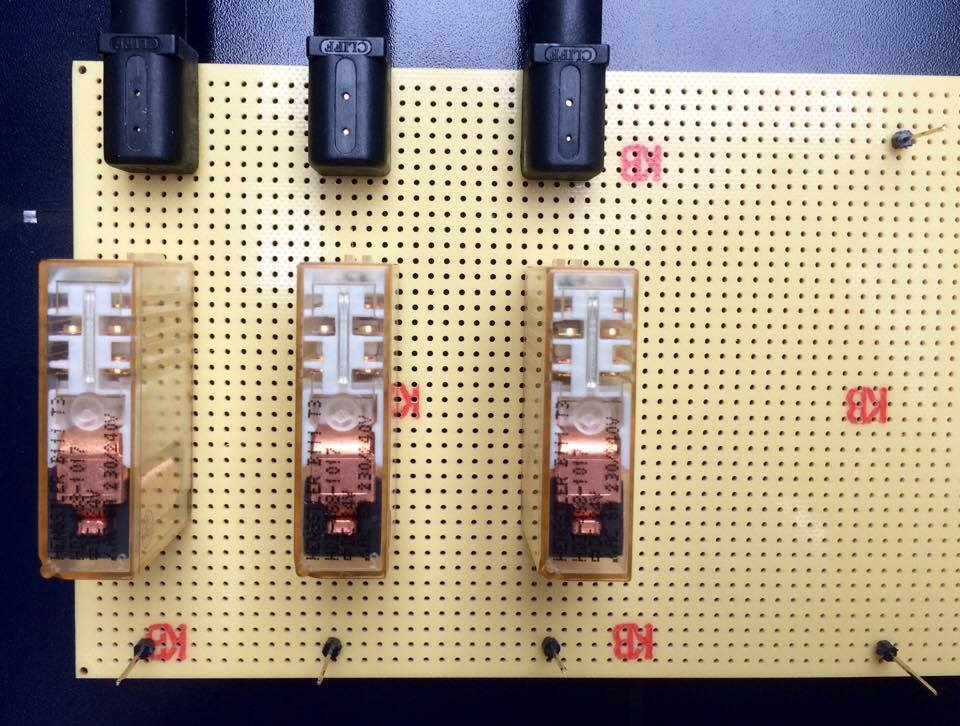
\includegraphics[width=0.6\textwidth]{figure/Relaekredsl}
	\caption{Færdigt print med relæer}
	\label{fig:Relae}
\end{figure}

\subsection{Implementering af Trinsskifter}
\label{sec:ImpTrinskift}
Trinskifter består af trintransformer og relækredsløb. På figur \ref{fig:Trinskift} ses, hvordan disse kobles til PLC, Distributionslinje og belastninger.

\begin{figure}[H]
	\centering
	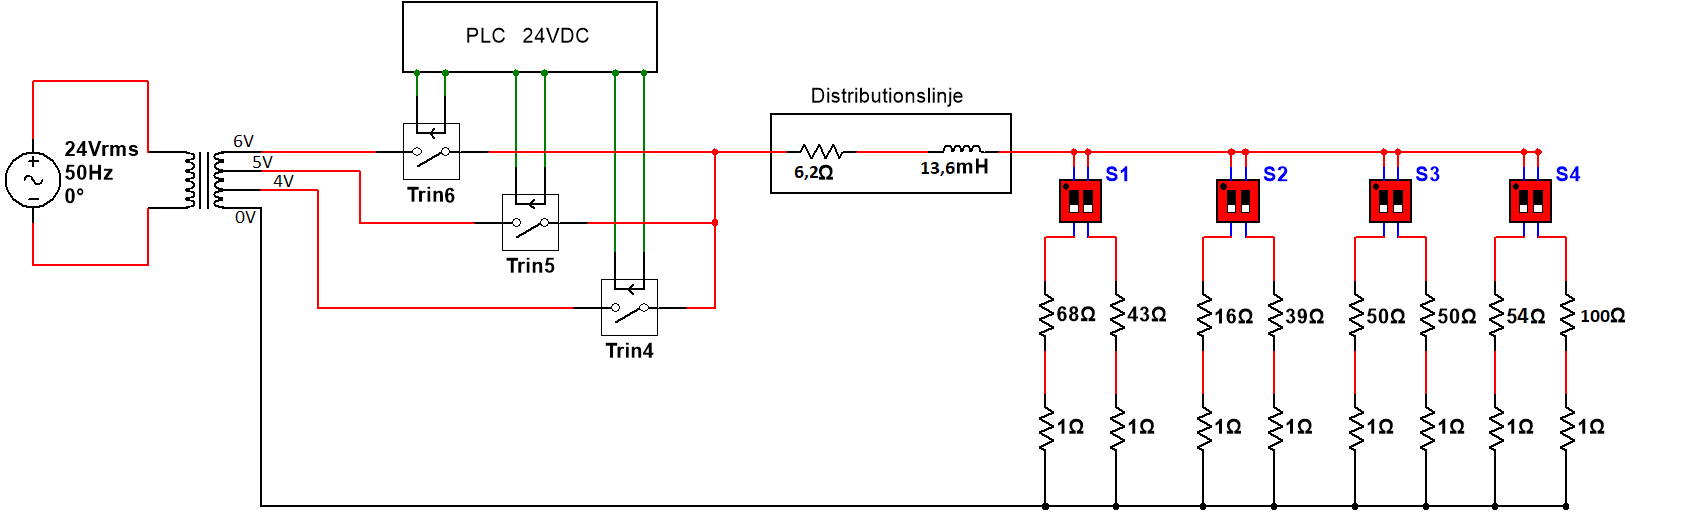
\includegraphics[width=0.9\textwidth]{figure/Trinskiftertegning2}
	\caption{Kredsløbstegning af Distributionslinje, belastninger og Trinskifter}
	\label{fig:Trinskift}
\end{figure}

Det ses, hvorledes hvert trin på transformeren er tilkoblet hvert kontaktrelæ. Gennem PLC styresignalet tilkobles ønsket trin. Eksempelvis for at skifte fra trin 4V til trin 5V, kobles trin 4V og trin 5V. Efter to sekunder slås trin 4V fra, og dermed bliver trin 5V det gældende trin. På denne måde sikres det, at forsyningen til systemet ikke forsvinder ved trinskift. Det er muligt at koble to trin på samme tid, da strømmen altid vil vælge den korteste vej i viklingerne på transformerens sekundærside. 



